\section{Autonomous Vehicles History}

\begin{frame}
\frametitle{History of Autonomous Vehicles Development}
\framesubtitle{The Early Years (1990s)}
Prometheus, etc.
\end{frame}

\begin{frame}
\frametitle{History of Autonomous Vehicles Development}
\framesubtitle{The DARPA Challenges (2004-2008)}
\begin{columns}[T]
    \begin{column}{.65\textwidth}
    DARPA Grand Challenges\footnotemark
    \begin{itemize}
        \item In the 2004 competition, 15 teams competed for a \$1 million prize
            on a 240 km desert route
        \item The prize went unclaimed; the best team was able to complete
            11.78 km
        \item In 2005, a \$2 million prize was up for grabs on a 212 km route
        \item The team from Stanford University with their vehicle
            \emph{Stanley} completed the course the fastest (in total 5 teams
            completed the course)
    \end{itemize}
    \end{column}
    \begin{column}{.35\textwidth}
    \centering
    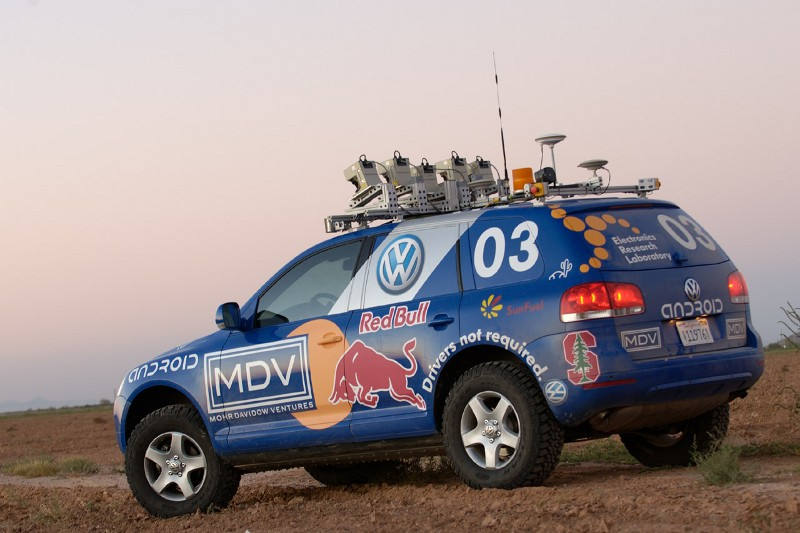
\includegraphics[height=2.5cm]{images/darpa_stanley.jpg} \\
    \tiny{\cite{DARPAStanley}}
    \end{column}
\end{columns}
\footnotetext[1]{\tiny{https://www.darpa.mil/about-us/timeline/-grand-challenge-for-autonomous-vehicles}}
\end{frame}
    
\begin{frame}
\frametitle{History of Autonomous Vehicles Development}
\framesubtitle{The DARPA Challenges (2004-2008)}
\begin{columns}[T]
    \begin{column}{.7\textwidth}
    DARPA Urban Challenge\footnotemark
    \begin{itemize}
        \item In 2007, a third competition for a \$2 million prize was held on
            a 96 km urban route
        \item A total of 11 teams competed in the final competition
        \item A team from Carnegie Melon University won with their vehicle
            \emph{Boss}
    \end{itemize}
    \end{column}
    \begin{column}{.3\textwidth}
    \centering
    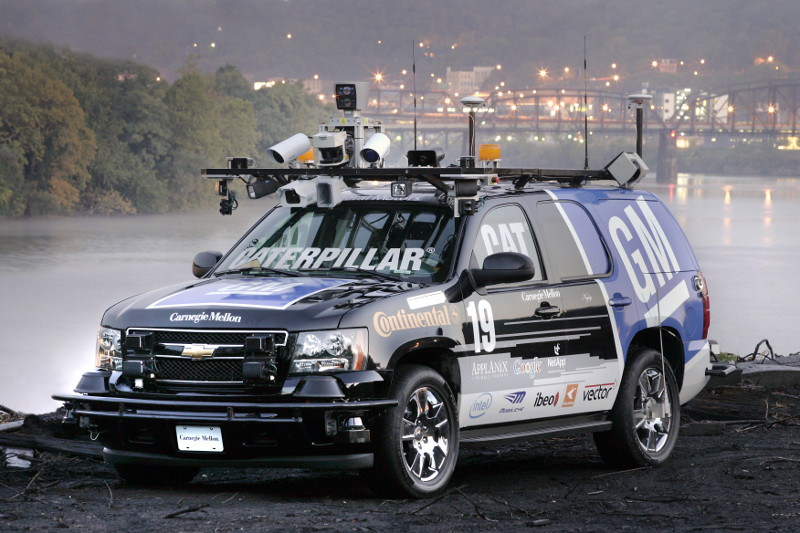
\includegraphics[height=2.25cm]{images/darpa_boss.jpg} \\
    \tiny{\cite{CMUUrbanChallenge}}
    \end{column}
\end{columns}
\begin{block}{Legacy}
The student, engineers, and companies of the DARPA challenges laid the
foundations for today's autonomous driving development and are leaders in the
industry.
\end{block}
\footnotetext[2]{\tiny{https://www.darpa.mil/about-us/timeline/darpa-urban-challenge}}
\end{frame}

\begin{frame}
\frametitle{History of Autonomous Vehicles Development}
\framesubtitle{The Industry Research Ramp-Up (2010-2020)}
OEMs, Tier 1s, and new companies ramping up
\end{frame}

\begin{frame}
\frametitle{History of Autonomous Vehicles Development}
\framesubtitle{Going to Production (2020 - )}
Commercial roll-outs happening today
\end{frame}